\section{Evaluierung der Modelle}\raggedbottom
\label{evalmetric}
Die unterschiedlichen Optimierungen der Latentvektoren für ein Optimus Modell und des Cellstates für \textsc{BiMeanVAE} werden auf dem Amazon und dem Yelp Datensatz verglichen und mit dem aktuellem State-of-the-Art Modell COOP in Relation gesetzt.
Es existieren im Dev-Datensatz und Test-Datensatz jeweils 8 Eingabebewertungen und drei Gold-Summaries zum Evaluieren der generierten Ausgabebewertungen.
Die Eingabebewertungen werden durch ein Optimus VAE Modell und ein \textsc{BiMeanVAE} Modell in Latentvektoren umgewandelt.
Anschließend werden mittels in Abschnitt \ref{coop_chap} dargestellter COOP Herangehensweise die Latentvektoren kombiniert, um den \textit{Input-Output-Overlap} zu maximieren. 
Weiterhin werden die Latentvektoren mittels in dieser Arbeit eingeführtem Attribut-Modell optimiert, um detailreiche und umfassende Durchschnittsrezensionen zu erhalten.


\subsection{Evaluationsmetriken}
Die generierten Textbewertungen werden mit den drei Gold-Summaries verglichen.
Zum Vergleich der generierten Rezensionen wird die ROUGE (\textbf{R}ecall-\textbf{O}riented \textbf{U}nderstudy for \textbf{G}isting \textbf{E}valuation)-Metrik verwendet \citep{lin-2004-rouge}.
Die ROUGE-N Metrik misst die Anzahl der übereinstimmenden N-Grams zwischen dem generierten Text und den Referenztexten. 
Ein N-Gram ist eine N-lange sequentielle Folge von Wörtern innerhalb der Texte. 

Zur Bewertung der generierten Rezensionen werden die vorhergesagten Ergebnisse mit den korrekten Ergebnissen verglichen. 
Die Konfusionsmatrix in Abbildung \ref{confusionmatrix} ist eine Wahrheitsmatrix, welche die Einteilung der vorhergesagten Ergebnisse ermöglicht. 
True Positive (TP) und True Negative (TN) sind von dem Modell korrekt vorhergesagte Ergebnisse, False Positive (FP) und False Negative (FN) ist eine Klasse von falsch vorhergesagten Ergebnissen.



\begin{figure}[h!]
    \centering
\begin{tikzpicture}[
    box/.style={draw,rectangle,minimum size=2cm,text width=1.5cm,align=left}]
    \matrix (conmat) [row sep=.1cm,column sep=.1cm] {
    \node (tpos) [box,
        label=left:Positive,
        label=above:Positive,
        ] {True \\ positive};
    &
    \node (fneg) [box,
        label=above:Negative] {False \\ negative};
    \\
    \node (fpos) [box,
        label=left:Negative] {False \\ positive};
    &
    \node (tneg) [box] {True \\ negative};
    \\
    };
    \node [left=.05cm of conmat,text width=1.5cm,align=right] {\textbf{Referenz}};
    \node [above=.05cm of conmat] {\textbf{Vorhersage}};
\end{tikzpicture}
\caption{Konfusionsmatrix zur Berechnung des ROUGE-N Scores}
\label{confusionmatrix}
\end{figure}

Zur Berechnung des ROUGE-N Scores werden die einzelnen Textabschnitte in eine Menge aus N-Grams zerlegt.
Mittels der Konfusionsmatrix in Abbildung \ref{confusionmatrix} lassen sich Precision (P) und Recall (R) definieren:
\begin{addmargin}[30pt]{30pt}
    \textbf{Precision}: 
    Der Precision Wert ergibt sich aus dem Verhältnis der korrekt vorhergesagten N-Grams und der Anzahl der insgesamt vorhergesagten N-Grams.
    \begin{align*}
    \text{P} = \frac{\text{TP}}{\text{TP}+\text{FP}}
    \end{align*}

    \textbf{Recall}:
    Recall ist als Verhältnis zwischen den korrekt vorhergesagten N-Grams und den N-Grams aus der Referenz definiert.
    \begin{align*}
    \text{R} = \frac{\text{TP}}{\text{TP}+\text{FN}}
    \end{align*}

    $\textbf{F}_\textbf{1}$:
    Das F1-Maß beschreibt das harmonische Mittel zwischen Precision und Recall.
    \begin{align*}
    \text{F}_\text{1} = \frac{2\text{PR}}{\text{P}+\text{R}}
    \end{align*}
\end{addmargin}

In der Evaluation werden die ROUGE-1, ROUGE-2 und ROUGE-L Werte miteinander verglichen.
ROUGE-1 verwendet als N-Gram Unigramme, ROUGE-2 Bigramme und ROUGE-L misst die längste gleiche Subsequenz zwischen Vorhersage und Referenz.

Da die ROUGE-Scores lediglich die einzelnen Wortsequenzen miteinander vergleichen, findet die semantische Bedeutung und Ähnlichkeit der Bewertungen mit der Referenz keinen Einfluss.
Hier erzielen zum Beispiel Synonyme keine guten ROUGE-Scores, obwohl sie eine semantische Übereinstimmung haben.
Um trotzdem die semantische Ähnlichkeit zwischen Bewertungen und Referenz zu messen, wird als weitere Metrik der Moverscore aus Abschnitt \ref{moverscore} verwendet.
Der Moverscore basiert auf BERT und vergleicht Context-Embeddings mittels Earth-Mover-Distance \citep{emd}. Als Metrik konnte der Moverscore hohe Korrelationen mit menschlichem Urteilsvermögen aufweisen.


\subsection{Moverscore}
\label{moverscore}
Der Moverscore \citep{moverscore_paper} ist eine Evaluationsmetrik, die semantische Inhalte zwischen zwei Textsequenzen vergleicht und diesen einen Ähnlichkeitswert zuweist.
Das Ziel vom Moverscore ist es eine Metrik abzubilden, die einer menschlichen Bewertung der Ähnlichkeit von zwei Sequenzen am nähesten ist. 
Im Gegensatz zu anderen Textähnlichkeitsmetriken, die lediglich die Überlappungen von Tokens innerhalb der Sequenzen messen ohne die Semantik der Wörter zu bewerten, 
bildet sich der Moverscore aus einer Kombination bestehend aus einer im Kontext eingebetteten Repräsentation der einzelnen Textsequenzen, die eine semantische Distanz untereinander abbilden.
Die semantische Distanz wird über die Word Mover Distance \citep{wordmoverdistance}, einer Metrik basierend auf der Earth Mover Distance, bestimmt. Es wird ein minimaler Transportfluss zwischen den einzelnen Sequenzen errechnet.
Die Worteinbettungen werden durch ein BERT Modell erzeugt.

Insgesamt ist der Moverscore für die Bewertungsgenerierung ein wichtiger Leistungsindikator, da nicht nur übereinstimmende N-Gramme an Wörtern gemessen werden, sondern die Semantik der einzeln Wörter miteinbezogen wird. 
Da insbesondere in Bewertungen ähnliche Meinungen auf unterschiedliche Weise ausgedrückt werden können, bietet sich der Moverscore hier gut als Metrik an, um diese Übereinstimmungen zu finden, siehe Abschnitt \ref{moverscore_ranking}.


% \subsection{Bewertung der Datensätze}

% \subsubsection{Amazon-Datensatz}

% \subsubsection{Yelp-Datensatz}

\subsection{Ergebnisse}
\label{eval_results_chapter}
In Tabelle \ref{eval_results} ist die Performance der unterschiedlichen untersuchten und erstellten Modelle dargestellt.
In dieser Arbeit wurde das \glqq \textit{COOP}+Attribute Model\grqq{} Modell entwickelt.
Es basiert auf dem \textit{COOP} Modell und verbessert die Generierung von neuen Rezensionen durch die Verwendung eines Attribut-Modells.
Unterschieden werden die \textit{COOP} Modelle durch ihre grundlegend verwendete Variational Autoencoder Architektur in Optimus und \textsc{BiMeanVAE}, siehe Kapitel \ref{vae}.
Das Optimus Modell kombiniert BERT und GPT-2 in einem Variational Autoencoder Modell. \textsc{BiMeanVAE} hingegen besteht aus einem BiLSTM Encoder mit einem LSTM Decoder trainiert als Variational Autoencoder Modell.

Verglichen wird die Performance der unterschieldichen Modelle mit den zuvor beschriebenen Evaluationsmetriken, dem ROUGE-1, ROUGE-2, ROUGE-L Score und dem Moverscore.
Diese Metriken lassen ausreichend Rückschlüsse auf die erreichte Performance der Modelle und einer Leistungssteigerung zwischen den \textit{COOP} Basismodellen und den modifizierten \textit{COOP} mit Attributionsmodellen zu.

\begin{table}[!h]
  
    \centering
    \begin{tabular}{@{}lcccc|cccc@{}}
    \toprule
             Test-Dataset                  & \multicolumn{4}{c}{Amazon} & \multicolumn{4}{c}{Yelp} \\ 
    \textbf{Method} & \textbf{R1} & \textbf{R2} & \textbf{RL} & \textbf{MV} & \textbf{R1} & \textbf{R2} & \textbf{RL} & \textbf{MV}\\ \midrule
    % \textit{COOP + Attribute Model - DEV Scores}        &         &         &        &        &        &   & &     \\
    % $\quad$ Optimus            &     \textbf{37.01}    &   \underline{7.44}  &  20.55  & \textbf{23.86} &   \textbf{35.99}   &   \textbf{7.79}       & \underline{19.40}   &   23.56 \\ 
    % $\quad$ \textsc{BiMeanVae}   &   \underline{36.47}   &   \textbf{7.59}    &   \textbf{22.22}  & 23.05 &     &      &   &    \\ \midrule
    
    \textit{COOP + Attribute Model}        &         &         &        &        &        &   & &     \\
    $\quad$ Optimus   ?         &   35.57   & 7.50  &  20.28 & 56.49 &     &         &   &    \\ 
    $\quad$ \textsc{BiMeanVae}   &   \textbf{37.94}  &   7.20    &  \textbf{21.75} & \textbf{56.69} &     &      &   &    \\ \midrule
    


    \textit{COOP}              &         &         &        &        &        & &   &    \\ %PAPER
    $\quad$ Optimus           & 35.32 &6.22 &19.84  & 56.41&  33.68& 7.00 &18.95 & 56.41\\ 
    $\quad$ \textsc{BiMeanVae}  & 36.57 &7.23 &21.24 & 56.49 & 35.37& 7.35 &19.94 & 56.78\\ \midrule
    

    % \textit{COOP}              &         &         &        &        &        & &   &    \\
    % $\quad$ Optimus           & 33.60  & 6.63    & 20.87 & \underline{20.85} & 33.60  & 7.00   & 18.95 & 56.41\\ 
    % $\quad$ \textsc{BiMeanVae}  & 36.40 &  7.16 &  21.08 & 56.49 & 35.37  & \underline{7.35}  & \textbf{19.94} & 56.78\\ \midrule
    
    % \textit{COOP-DEV}              &         &         &        &        &        & &   &    \\
    % $\quad$ Optimus $^{\star}$           & 35.32   & 6.22    & 19.84 & \underline{23.22} & 33.60  & 7.00   & 18.95 & 23.33\\ 
    % $\quad$ \textsc{BiMeanVae}$^{\dagger}$  & $\text{35.67}^{\dagger}$    & $\text{6.53}^{\dagger}$   & \underline{$\text{21.07}^{\dagger}$} & 22.12 & \underline{35.37}  & \underline{7.35}  & \textbf{19.94} & 23.78\\ \midrule
    

    \textit{SimpleAvg}                   &         &         &       &      &        &        &        \\
    $\quad$ Optimus  $^{\star}$          & 33.54   & 6.18    & 19.34 & 22.35& 31.23  & 6.48   & 18.27 & 23.05\\
    $\quad$ \textsc{BiMeanVae}$^{\star}$ & 33.60   & 6.64    & 20.87 & 20.85& 32.87  & 6.93   & 19.89 & 22.41\\
    $\quad$ CopyCat  $^{\star}$          & 31.97   & 5.81    & 20.16 &-     & 29.47  & 5.26   & 18.09 & -\\ 
    $\quad$ MeanSum  $^{\star}$          & 29.20   & 4.70    & 18.15 & -    & 28.46  & 3.66   & 15.57 & -\\ \midrule
    \textit{Extractive}                  &         &         &       &      &        &        &       &      \\
    $\quad$ LexRank  $^{\star}$          & 28.74   & 5.47    & 16.75 & -    & 25.01  & 3.62   & 14.67 & -\\ \bottomrule
    \end{tabular}
    \caption{ROUGE und Moverscore Ergebnisse auf den Test-Benchmarkdatensätzen der unterschiedlichen Modelle. Die besten Ergebnisse sind fett markiert und die zweitbesten Ergebnisse unterstrichen.
    Der Stern $^{\star}$ denotiert, dass die ROUGE-Ergebnisse aus den Ergebnissen von \citep{coop} übernommen wurden.
    %$^{\dagger}$ Evaluierte Performance unterscheidet sich vom \citep{coop} Paper. Performance wurde nach SourceCode des Papers bestimmt.
    }
    \label{eval_results}
\end{table}

Grundsätzlich lassen sich die Ergebnisse in Tabelle \ref{eval_results} in die Kategorien abstraktive und extraktive Zusammenfassung unterteilen.
Hier ist eindeutig zu erkennen, dass LexRank als extraktive Methode in allen Bereichen den abstraktiven Methoden unterliegt. 
Die Gruppe der abstraktiven Methoden umfasst die \textit{SimpleAVG} Gruppe, die \textit{COOP} Gruppe und die \textit{COOP+Attribute Model} Gruppe, die alle auf Variational Autoencoder basieren.
Diese Gruppen wurden nach der Kombinationsmethode der einzelnen Latentvektoren zu einem repräsentativen Latentvektor unterschieden.


Die \textit{SimpleAvg} Gruppe umfasst unterschiedliche abstraktive Textzusammenfassungsmethoden auf Basis von Variational Autoencodern.
Bei dieser Gruppe wird von allen erzeugten Latentvektoren ein normaler Durchschnittsvektor errechnet, von dem anschließend gesamplet wird.
Es ist erkennbar, dass die beiden Methoden Optimus und \textsc{BiMeanVAE} den Methoden CopyCat und MeanSum überlegen sind, da diese in allen Messwerten bessere Ergebnisse erzielen.
Besonders hervozuheben ist hier, dass Optimus bessere Moverscore Ergebnisse als \textsc{BiMeanVAE} erzielt, allerdings in den ROUGE Werten minimal schlechter abschneidet. 

Eine große Leistungssteigerung ergibt sich durch die \textit{COOP} Methode, die eine optimale Kombination der einzelnen Latentvektoren findet.
Hier erzielen sowohl Optimus als auch \textsc{BiMeanVAE} in allen Metriken bessere Ergebnisse als die \textit{SimpleAvg} Vergleichsgruppe.
Demnach ist das Durchsuchen der Kombinationen von Latentvektoren sinnvoll. 
Insbesondere der ROUGE-1 Score übertrifft die \textit{SimpleAVG} Scores bei Optimus und \textsc{BiMeanVAE} signifikant im Durchschnitt um 1.93\%.  %PROZENT COOP-SIMPLEAVG
Die größte Leistungssteigerung zwischen der \textit{COOP} Kombinationsstrategie und \textit{SimpleAvg} erfährt \textsc{BiMeanVAE}.
Dies ist sehr beeindruckend, da \textit{BiMeanVAE} mit 13 Millionen Parametern weitaus weniger Parameter hat als Optimus mit 239 Millionen Parametern und auch nicht auf vortrainierte Sprachmodelle zurückgreifen kann.
Demnach lassen sich mittels Variational Autoencoder Textsequenzen hervorragend in Latentvektoren encodieren und diese mittels Vektoroperationen kombinieren.


%Vergleich Optimus vs BiMeanVAE an Texten
Eine weitere Leistungssteigerung der verwendeten Variational Autoencoder Optimus und \textsc{BiMeanVAE} mit \textit{COOP} Kombinatorik lässt sich durch die in dieser Arbeit verwendeten Attributmodelle feststellen.
Die aus dem Latentvektoren decodierten Textsequenzen lassen sich so noch stärker in die gewünschte Richtung bei der Generierung adaptieren. 
Das verwendete Attributmodell ist ein Bag of Words Modell, welches aus den 150 am häufigsten vorkommenden Tokens besteht. 
Somit wird die Gewichtung bei der Generierung auf die häufig vorkommenden Tokens gelenkt und die generierten Textsequenzen haben eine höhere Überlappung.
Beispielsweise fällt auf, dass beim Generieren teilweise mehrere vorgeschlagene Tokens ein hohes Ranking erhalten, wobei am Ende durch das Attributionsmodell das am besten passende mit einer höheren Wahrscheinlichkeit ausgewählt wird.
Insbesondere spezifische Begriffe die ausschlaggebend für die erzeugten Rezensionen sind, allerdings in einer normalen Sprachverteilung eine geringe Gewichtung erhalten würden, werden durch das Bag of Words Attributmodell stark hervorgehoben.

Die Performance des kombinierten \textit{COOP + Attributmodells} zeigt in den ROUGE-1 Scores in allen Modellen deutliche Verbesserungen gegenüber den normalen \textit{COOP} Modellen.


\subsection{Beispiele für generierte Rezensionen}


\small
%Define a reference depth. 
%You can choose either relative or absolute.
%--------------------------
\newlength{\DepthReference}
\settodepth{\DepthReference}{g}%relative to a depth of a letter.
\setlength{\DepthReference}{1pt}%absolute value.

%Define a reference Height. 
%You can choose either relative or absolute.
%--------------------------
\newlength{\HeightReference}
\settoheight{\HeightReference}{T}
\setlength{\HeightReference}{7pt}


%--------------------------
\newlength{\Width}%

\newcommand{\ccolorbox}[2][red]%
{%
    \settowidth{\Width}{#2}%
    \setlength{\fboxsep}{1pt}%
    \colorbox{#1}%
    {%      
        \raisebox{-\DepthReference}%
        {%
                \parbox[b][\HeightReference+\DepthReference][c]{\Width}{\centering#2}%
        }%
    }%
}



\definecolor{HighlightColor}{HTML}{dc2626}
\definecolor{BackgroundColor}{HTML}{bfdbfe}
\normalsize


Folgend werden einige generierte Textrezensionen des COOP Modells und des COOP + Attributionsmodell Modells direkt miteinander verglichen.
Es wurden jeweils zwei generierte Rezensionen des COOP und des COOP + Attributionsmodell Modells zu den Datensätzen Amazon und Yelp ausgewählt. 
Zur besseren Darstellung sind bei den generierten Rezensionen die mit der Gold-Zusammenfassung übereinstimmenden Unigrams \textcolor{HighlightColor}{rot} markiert, Bigrams sind \ccolorbox[BackgroundColor]{farblich blau hinterlegt} und die längste übereinstimmende Textsequenz \underline{unterstrichen}.
Der Moverscore lässt sich nicht visualisieren.

Authentische Rezensionen sollten konsistent in ihrem Inhalt sein, präzise auf Eigenschaften und Aspekte der Produkte oder Dienstleistungen eingehen und der Inhalt der generierten Rezension sollte mit den Eingabebewertungen deckungsgleich sein.
Anhand dieser Kriterien werden nachfolgend mehrere generierte Rezensionen bewertet.

% \setlength{\DepthReference}{6pt}
% \setlength{\HeightReference}{6pt}

\setlength{\fboxsep}{0.7em}

\subsubsection{Amazon Rezensionen}
Nachfolgend werden zwei generierte Rezensionen des Amazon Datensatzes evaluiert.
\begin{Rezension}[!h]
    \centering
    %\scriptsize
    \small
    \framebox{
        \parbox{\columnwidth-4\fboxsep}{
            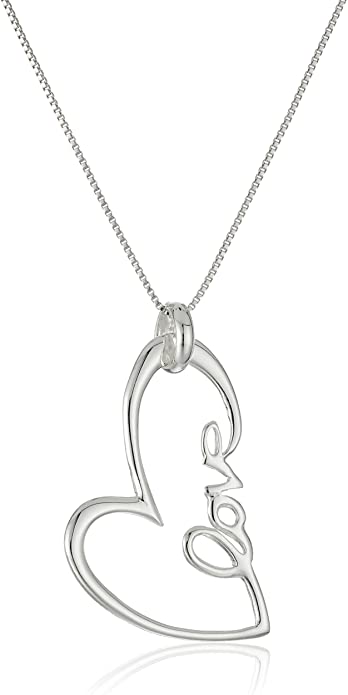
\includegraphics[width=1.3cm]{bilder/necklace.jpg} \textbf{Produkt:} Sterling Silver \glqq{}Love\grqq{} Open Heart Pendant Necklace, 18\grqq{} \\ \\
        \textbf{\textsc{BiMeanVAE} COOP+Attribute-Model:} \ccolorbox[BackgroundColor]{ \textcolor{HighlightColor}{\strut This necklace}} \ccolorbox[BackgroundColor]{ \textcolor{HighlightColor}{\strut is a}} \ccolorbox[BackgroundColor]{ \textcolor{HighlightColor}{\strut great quality}} \textcolor{HighlightColor}{and} \textcolor{HighlightColor}{so} \textcolor{HighlightColor}{far} \textcolor{HighlightColor}{it} \textcolor{HighlightColor}{'s} are \textcolor{HighlightColor}{the} perfect \textcolor{HighlightColor}{size} \ccolorbox[BackgroundColor]{ \textcolor{HighlightColor}{\strut . It}} \ccolorbox[BackgroundColor]{ \textcolor{HighlightColor}{\strut is a}} \textcolor{HighlightColor}{very} \textcolor{HighlightColor}{nice} \textcolor{HighlightColor}{looking} \textcolor{HighlightColor}{necklace} \textcolor{HighlightColor}{,} \ccolorbox[BackgroundColor]{ \textcolor{HighlightColor}{\strut and the}} color \underline{\ccolorbox[BackgroundColor]{ \textcolor{HighlightColor}{\strut is beautiful}} \ccolorbox[BackgroundColor]{ \textcolor{HighlightColor}{\strut . The}} \ccolorbox[BackgroundColor]{ \textcolor{HighlightColor}{\strut chain is}} \textcolor{HighlightColor}{a}} perfect gift \ccolorbox[BackgroundColor]{ \textcolor{HighlightColor}{\strut for the}} \textcolor{HighlightColor}{price} \textcolor{HighlightColor}{of} \textcolor{HighlightColor}{the} necklace. I love \textcolor{HighlightColor}{it} \textcolor{HighlightColor}{!} \\ 
        \textbf{Scores:} R-1: 48.63, R-2: 16.78, R-L: 28.08, MV: 60.05\\ \\
        \textbf{\textsc{BiMeanVAE} COOP:} \textcolor{HighlightColor}{This} \ccolorbox[BackgroundColor]{ \textcolor{HighlightColor}{\strut is a}} \textcolor{HighlightColor}{great} product \underline{\ccolorbox[BackgroundColor]{ \textcolor{HighlightColor}{\strut for the}} \ccolorbox[BackgroundColor]{ \textcolor{HighlightColor}{\strut price .}}} \textcolor{HighlightColor}{It} \ccolorbox[BackgroundColor]{ \textcolor{HighlightColor}{\strut is a}} \textcolor{HighlightColor}{very} \textcolor{HighlightColor}{good} \textcolor{HighlightColor}{quality} \textcolor{HighlightColor}{,} \ccolorbox[BackgroundColor]{ \textcolor{HighlightColor}{\strut and the}} \textcolor{HighlightColor}{price} was right \ccolorbox[BackgroundColor]{ \textcolor{HighlightColor}{\strut . The}} only thing \textcolor{HighlightColor}{is} that \ccolorbox[BackgroundColor]{ \textcolor{HighlightColor}{\strut it is}} \textcolor{HighlightColor}{a} little small \ccolorbox[BackgroundColor]{ \textcolor{HighlightColor}{\strut , but}} \textcolor{HighlightColor}{it} \textcolor{HighlightColor}{'s} not too big \ccolorbox[BackgroundColor]{ \textcolor{HighlightColor}{\strut . It}} \textcolor{HighlightColor}{'s} \ccolorbox[BackgroundColor]{ \textcolor{HighlightColor}{\strut a great}} buy \ccolorbox[BackgroundColor]{ \textcolor{HighlightColor}{\strut for the}} \ccolorbox[BackgroundColor]{ \textcolor{HighlightColor}{\strut price .}}  \\ 
        \textbf{Scores:} R-1: 36.61, R-2: 8.30, R-L: 26.44, MV: 55.57 \\ \\
    
        \textbf{Optimus COOP+Attribute-Model:} \textcolor{HighlightColor}{This} \ccolorbox[BackgroundColor]{ \textcolor{HighlightColor}{\strut is a}} \textcolor{HighlightColor}{great} gift \underline{\ccolorbox[BackgroundColor]{ \textcolor{HighlightColor}{\strut for the}} \ccolorbox[BackgroundColor]{ \textcolor{HighlightColor}{\strut price .}}} She loves \textcolor{HighlightColor}{it} \textcolor{HighlightColor}{,} \textcolor{HighlightColor}{so} much better than \textcolor{HighlightColor}{the} \textcolor{HighlightColor}{necklace} \textcolor{HighlightColor}{and} \textcolor{HighlightColor}{it} looks \ccolorbox[BackgroundColor]{ \textcolor{HighlightColor}{\strut beautiful .}} You ca \textcolor{HighlightColor}{n't} \textcolor{HighlightColor}{get} \textcolor{HighlightColor}{a} gift on \ccolorbox[BackgroundColor]{ \textcolor{HighlightColor}{\strut the chain}} \ccolorbox[BackgroundColor]{ \textcolor{HighlightColor}{\strut , but}} \ccolorbox[BackgroundColor]{ \textcolor{HighlightColor}{\strut it is}} not worth \textcolor{HighlightColor}{the} money \textcolor{HighlightColor}{!} \textcolor{HighlightColor}{It} looks \textcolor{HighlightColor}{great} \textcolor{HighlightColor}{!}         \\ 
        \textbf{Scores:} R-1: 42.65, R-2: 9.28, R-L: 26.57, MV: 58.31\\ \\
        \textbf{Optimus COOP:}  \ So \textcolor{HighlightColor}{far} \textcolor{HighlightColor}{the} \underline{\ccolorbox[BackgroundColor]{ \textcolor{HighlightColor}{\strut necklace is}} \textcolor{HighlightColor}{beautiful}} \textcolor{HighlightColor}{,} \ccolorbox[BackgroundColor]{ \textcolor{HighlightColor}{\strut and the}} perfect gift \textcolor{HighlightColor}{for} someone who \ccolorbox[BackgroundColor]{ \textcolor{HighlightColor}{\strut is a}} \ccolorbox[BackgroundColor]{ \textcolor{HighlightColor}{\strut beautiful piece}} \ccolorbox[BackgroundColor]{ \textcolor{HighlightColor}{\strut . It}} looks \textcolor{HighlightColor}{great} on \textcolor{HighlightColor}{the} picture \ccolorbox[BackgroundColor]{ \textcolor{HighlightColor}{\strut , but}} \textcolor{HighlightColor}{it} does not \textcolor{HighlightColor}{look} like \textcolor{HighlightColor}{a} gift \textcolor{HighlightColor}{.} Im \textcolor{HighlightColor}{very} happy with \textcolor{HighlightColor}{this} \textcolor{HighlightColor}{necklace} \textcolor{HighlightColor}{and} \ccolorbox[BackgroundColor]{ \textcolor{HighlightColor}{\strut it is}} not worth \textcolor{HighlightColor}{the} money \textcolor{HighlightColor}{!}  \\ 
        \textbf{Scores:} R-1: 40.26, R-2: 13.01, R-L: 23.48, MV: 58.06 }
    
        }
    \caption{Vergleich der generierten Rezensionen zwischen dem \textsc{BiMeanVAE} COOP und COOP + Attributionsmodell zu Produkt B0040EIHQQ des Amazon Datensatzes}
\label{reviewAmz1}
\end{Rezension}

Die in Rezension \ref{reviewAmz1} generierten Bewertungen für eine Halskette des Amazons Datensatzes zeigen konsistente Ergebnisse in beiden durch \textsc{BiMeanVAE} generierten Rezensionen. 
Das Sentiment ist positiv und die Kette wird abschließend zum Kaufen empfohlen. Besonders auffällig ist die höhere Präzision des Attributmodells. Das Produkt und die Eigenschaften dieses werden explizit erwähnt, wie zum Beispiel \glqq{}great quality\grqq{}, \glqq{}perfect size\grqq{}, \glqq{}very nice looking necklace\grqq{}, \glqq{}color is beautiful\grqq{} und \glqq{}perfect gift for the price\grqq{}.
Im Gegensatz dazu erwähnt das COOP Modell lediglich die Qualität \glqq{}great product\grqq{}, \glqq{}very good quality\grqq{} und den Preis \glqq{}price was right\grqq{}, \glqq{}great buy for the price\grqq{} des Produktes ohne auf spezifische Eigenschaften des Produktes wie Farbe oder Stil einzugehen.
Diese Auswertung spiegelt sich auch in den Metriken wieder, in denen das Attributmodell die Metriken des COOP Modells in allen Werten übertrifft. 
Insbesondere der Moverscore, der die semantische Ähnlichkeit zu den Gold-Zusammenfassungen angibt, ist mit 60.05 beim Attributmodell bedeutend höher als die 55.57 des COOP Modells.

Bei den durch Optimus erstellten Rezensionen widerspricht sich das positive Sentiment mit Beschreibungen wie \glqq{}perfect gift\grqq{} und anschließend keiner Kaufempfehlung \glqq{}it is not worth the money!\grqq{}.
Trotzdem gehen beide Modelle auf unterschiedliche Aspekte der zu bewertenden Kette ein und beschreiben den Stil der Kette als \glqq{}it looks beautiful\grqq{} und \glqq{}necklace is beautiful\grqq{}.
Eine Steigerung der Leistung der generierten Rezensionen des Attributmodells gegenüber dem COOP Modell kann hier nur an den Metriken festgestellt werden (außer in ROUGE-2) und spiegelt sich allerdings nicht in den generierten Rezensionen wieder.

\begin{Rezension}[!h]
    \centering
    %\scriptsize
    \small
    \framebox{
        \parbox{\columnwidth-4\fboxsep}{
            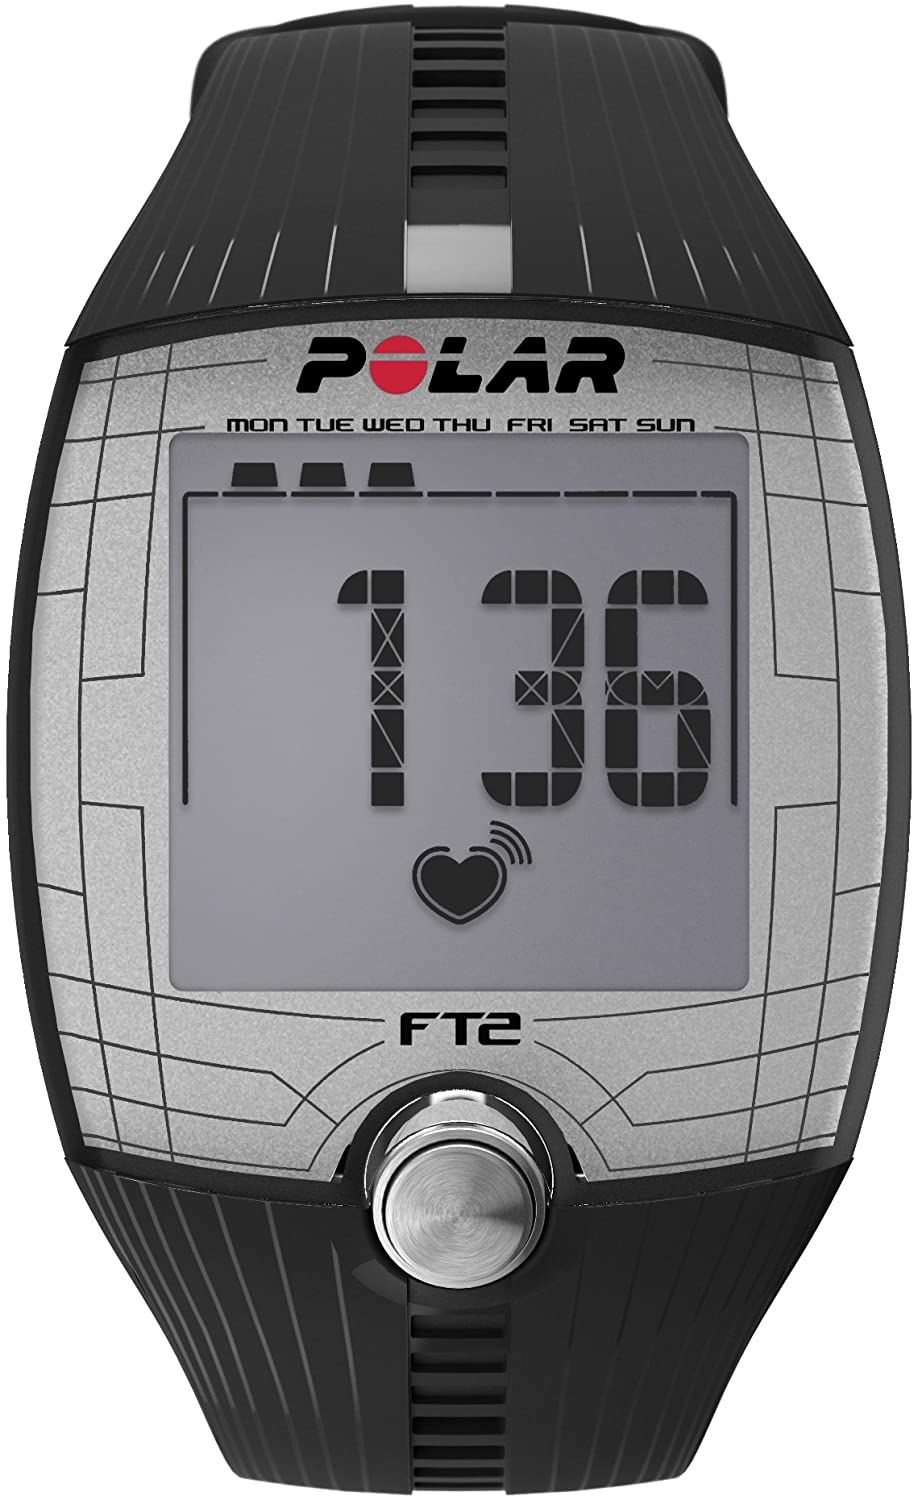
\includegraphics[width=1.5cm]{bilder/polarfit.jpg} \textbf{Produkt:} Polar FT2 Heart Rate Monitor \\ \\
        \textbf{\textsc{BiMeanVAE} COOP+Attribute-Model:} If \ccolorbox[BackgroundColor]{ \textcolor{HighlightColor}{\strut you are}} looking \textcolor{HighlightColor}{for} \underline{\ccolorbox[BackgroundColor]{ \textcolor{HighlightColor}{\strut a heart}} \ccolorbox[BackgroundColor]{ \textcolor{HighlightColor}{\strut rate monitor}}} \textcolor{HighlightColor}{this} \ccolorbox[BackgroundColor]{ \textcolor{HighlightColor}{\strut is the}} best \ccolorbox[BackgroundColor]{ \textcolor{HighlightColor}{\strut . It}} 's \ccolorbox[BackgroundColor]{ \textcolor{HighlightColor}{\strut easy to}} \textcolor{HighlightColor}{use} \textcolor{HighlightColor}{,} \textcolor{HighlightColor}{and} \textcolor{HighlightColor}{it} works great \ccolorbox[BackgroundColor]{ \textcolor{HighlightColor}{\strut . The}} \textcolor{HighlightColor}{only} downside \textcolor{HighlightColor}{is} \textcolor{HighlightColor}{that} \textcolor{HighlightColor}{you} have \textcolor{HighlightColor}{to} \textcolor{HighlightColor}{be} careful \textcolor{HighlightColor}{not} \textcolor{HighlightColor}{to} take \textcolor{HighlightColor}{it} \ccolorbox[BackgroundColor]{ \textcolor{HighlightColor}{\strut out of}} \textcolor{HighlightColor}{the} \textcolor{HighlightColor}{case} \textcolor{HighlightColor}{.} \\ 
        \textbf{Scores:} R-1: 39.26, R-2: 13.12, R-L: 22.08, MV: 56.40\\ \\
        \textbf{\textsc{BiMeanVAE} COOP:} \ccolorbox[BackgroundColor]{ \textcolor{HighlightColor}{\strut This is}} \textcolor{HighlightColor}{a} great \textcolor{HighlightColor}{product} \ccolorbox[BackgroundColor]{ \textcolor{HighlightColor}{\strut . It}} was \ccolorbox[BackgroundColor]{ \textcolor{HighlightColor}{\strut easy to}} \ccolorbox[BackgroundColor]{ \textcolor{HighlightColor}{\strut set up}} \textcolor{HighlightColor}{and} \ccolorbox[BackgroundColor]{ \textcolor{HighlightColor}{\strut use .}} \ccolorbox[BackgroundColor]{ \textcolor{HighlightColor}{\strut The only}} downside \textcolor{HighlightColor}{is} \textcolor{HighlightColor}{that} \textcolor{HighlightColor}{it} 's \textcolor{HighlightColor}{a} little hard \textcolor{HighlightColor}{to} get \textcolor{HighlightColor}{on} \textcolor{HighlightColor}{and} off \ccolorbox[BackgroundColor]{ \textcolor{HighlightColor}{\strut , but}} \textcolor{HighlightColor}{it} 's \textcolor{HighlightColor}{not} \textcolor{HighlightColor}{a} problem \ccolorbox[BackgroundColor]{ \textcolor{HighlightColor}{\strut . It}} \underline{\ccolorbox[BackgroundColor]{ \textcolor{HighlightColor}{\strut is easy}} \ccolorbox[BackgroundColor]{ \textcolor{HighlightColor}{\strut to use}}} \textcolor{HighlightColor}{and} \textcolor{HighlightColor}{the} price \textcolor{HighlightColor}{is} right \textcolor{HighlightColor}{.}         \\ 
        \textbf{Scores:} R-1: 28.99, R-2: 7.83, R-L: 20.11, MV: 54.33 \\ \\

        \textbf{Optimus COOP+Attribute-Model:} \underline{\ccolorbox[BackgroundColor]{ \textcolor{HighlightColor}{\strut This is}} \ccolorbox[BackgroundColor]{ \textcolor{HighlightColor}{\strut a good}}} price \ccolorbox[BackgroundColor]{ \textcolor{HighlightColor}{\strut . You}} ca \textcolor{HighlightColor}{n't} \textcolor{HighlightColor}{be} able \ccolorbox[BackgroundColor]{ \textcolor{HighlightColor}{\strut to use}} \textcolor{HighlightColor}{it} \textcolor{HighlightColor}{in} \textcolor{HighlightColor}{your} \ccolorbox[BackgroundColor]{ \textcolor{HighlightColor}{\strut heart rate}} \ccolorbox[BackgroundColor]{ \textcolor{HighlightColor}{\strut monitor ,}} \textcolor{HighlightColor}{which} \ccolorbox[BackgroundColor]{ \textcolor{HighlightColor}{\strut is very}} \textcolor{HighlightColor}{accurate} \textcolor{HighlightColor}{.} If \ccolorbox[BackgroundColor]{ \textcolor{HighlightColor}{\strut you need}} \textcolor{HighlightColor}{to} \textcolor{HighlightColor}{be} aware \textcolor{HighlightColor}{that} \textcolor{HighlightColor}{you} have \ccolorbox[BackgroundColor]{ \textcolor{HighlightColor}{\strut to read}} all \textcolor{HighlightColor}{the} reviews \textcolor{HighlightColor}{and} \textcolor{HighlightColor}{it} 's \textcolor{HighlightColor}{very} comfortable \ccolorbox[BackgroundColor]{ \textcolor{HighlightColor}{\strut . It}} \ccolorbox[BackgroundColor]{ \textcolor{HighlightColor}{\strut is easy}} \textcolor{HighlightColor}{to} \ccolorbox[BackgroundColor]{ \textcolor{HighlightColor}{\strut set up}} \textcolor{HighlightColor}{and} \textcolor{HighlightColor}{you} \textcolor{HighlightColor}{can} \textcolor{HighlightColor}{use} \textcolor{HighlightColor}{the} \ccolorbox[BackgroundColor]{ \textcolor{HighlightColor}{\strut monitor .}} \\ 
        \textbf{Scores:} R-1: 42.73, R-2: 12.25, R-L: 24.65, MV: 57.76 \\ \\
        \textbf{Optimus COOP:} \textcolor{HighlightColor}{It} 's \ccolorbox[BackgroundColor]{ \textcolor{HighlightColor}{\strut very} \underline{\textcolor{HighlightColor}{easy}}}\underline{ \ccolorbox[BackgroundColor]{ \textcolor{HighlightColor}{\strut to use}}} \textcolor{HighlightColor}{.} After reading \textcolor{HighlightColor}{the} reviews \textcolor{HighlightColor}{and} \ccolorbox[BackgroundColor]{ \textcolor{HighlightColor}{\strut it is}} \textcolor{HighlightColor}{very} \textcolor{HighlightColor}{accurate} \textcolor{HighlightColor}{.} If \textcolor{HighlightColor}{you} 're looking \textcolor{HighlightColor}{for} \textcolor{HighlightColor}{a} regular basis \textcolor{HighlightColor}{,} \textcolor{HighlightColor}{you} \textcolor{HighlightColor}{can} see \ccolorbox[BackgroundColor]{ \textcolor{HighlightColor}{\strut if you}} \textcolor{HighlightColor}{need} \textcolor{HighlightColor}{to} change \textcolor{HighlightColor}{the} \ccolorbox[BackgroundColor]{ \textcolor{HighlightColor}{\strut monitor .}} \textcolor{HighlightColor}{The} \ccolorbox[BackgroundColor]{ \textcolor{HighlightColor}{\strut monitor is}} \textcolor{HighlightColor}{that} \textcolor{HighlightColor}{it} 's \textcolor{HighlightColor}{not} too bulky \ccolorbox[BackgroundColor]{ \textcolor{HighlightColor}{\strut . Very}} happy \textcolor{HighlightColor}{with} \ccolorbox[BackgroundColor]{ \textcolor{HighlightColor}{\strut this product}} \textcolor{HighlightColor}{and} \textcolor{HighlightColor}{will} \textcolor{HighlightColor}{be} reccomend \textcolor{HighlightColor}{it} \textcolor{HighlightColor}{.}  \\ 
        \textbf{Scores:} R-1: 38.67, R-2: 8.98, R-L: 22.09, MV: 57.13 }
    
    }
    \caption{Vergleich der generierten Rezensionen zwischen dem \textsc{BiMeanVAE} COOP und COOP+Attributmodell zu Produkt B003HT9W32 des Amazon Datensatzes}
    \label{reviewAmz2}
\end{Rezension}


Rezension \ref{reviewAmz2} bewertet eine Fitness Puls Uhr des Amazon Datensatzes.
Die durch \textsc{BiMeanVAE} generierten Rezensionen sind in ihrem Inhalt konsistent und haben ein positives Sentiment. 
Beide Rezensionen erwähnen ähnliche Eigenschaften der Bedienungsfreundlichkeit \glqq{}easy to use\grqq{}, \glqq{}easy to setup and use\grqq{} und der Funktionalität \glqq{}it works great\grqq{}, \glqq{}great product\grqq{}.
Ebenfalls erwähnen beide generierten Rezensionen jeweils einen validen negativen Punkt der Fitness Uhr.
Somit gehen die Rezensionen präzise auf die Aspekte der Fitness Uhr ein. 
Die durch das Attributmodell generierte Rezension erwähnt, dass es sich um einen \glqq{}heart rate monitor\grqq{} handelt, wodurch diese Rezension noch präziser ist.
Dies ist auch in den Metriken zu erkennen, in denen das Attributmodell in allen Metriken eine bessere Leistung als das COOP Modell erzielt.

Die durch Optimus erzeugten Rezensionen haben eine schlechtere Konsistenz im Inhalt. 
Hier existieren sinnvolle Teilbereiche die auf Eigenschaften eingehen wie zum Beispiel \glqq{}is very accurate\grqq{}, allerdings wiedersprechen sich in beiden Rezensionen einige Fakten und bauen nicht konsistent aufeinander auf.
Beide Rezensionen erwähnen, dass es sich bei dem Produkt um einen \glqq{}heart rate monitor\grqq{} handelt.
Trotz der manuell evaluierten schlechteren Konsistenz des Inhaltes weisen beide Rezensionen bessere Metriken auf als die \textsc{BiMeanVAE} Modelle, wobei auch hier bei den Optimus Modellen das Attributmodell die besten Metriken erzielt. 
Wie auch bei Rezension \ref{reviewAmz1} zeigt hier das Attributmodell bei Optimus lediglich eine äußerst geringe Leistungssteigerung in der manuellen Evaluation, da zwar durch das Attributmodell spezielle Wörter wie \glqq{}heart rate monitor\grqq{} im Gegensatz zu \glqq{}monitor\grqq{} forciert werden, die Rezensionen trotzdem aber noch inkonsistent im Inhalt sind.

Insgesamt zeigt auf dem Amazon Datensatz das Attributmodell mit \textsc{BiMeanVAE} auf beiden Rezensionen \ref{reviewAmz1} und \ref{reviewAmz2} die besten Ergebnisse in Bezug auf konsistenten Inhalt und präzisen Formulierungen der wichtigen Aspekte der Produkte.
Durch das Attributmodell sind die \textsc{BiMeanVAE} Rezensionen wesentlich ausdrucksstärker, da seltene Wörter, die in Bezug auf die Rezensionen eine hohe Relevanz haben häufiger miteinbezogen werden.

\pagebreak
\subsubsection{Yelp Rezensionen}
Nachfolgend werden zwei generierte Rezensionen des Yelp Datensatzes evaluiert.
\begin{figure}[!h]
    \centering
    \scriptsize
    \framebox{

        \parbox{\columnwidth-4\fboxsep}{\textbf{Restaurant Id:} 87YsVbCN\_kfzheY79Fzjkg \\ \textbf{Review:} Great experience! Went cake tasting for our wedding and Jessica was a huge help!! She brought out the tastings for us after giving us time to look through their amazing book. She explained every cake and filling and had great recommendations for mixing the fillings. The champagne cake with cream cheese filling was amazing!! Chose our cake and design within an hour. Great service and knowledge. Thank you Jessica!}

    }
    \caption{Vergleich der Generierten Rezensionen zu einem Restaurant des Yelp Datensatzes}
\end{figure}
Lorem ipsum dolor sit amet, consetetur sadipscing elitr, sed diam nonumy eirmod tempor invidunt ut labore et dolore magna aliquyam erat, sed diam voluptua. At vero eos et accusam et justo duo dolores et ea rebum. Stet clita kasd gubergren, no sea takimata sanctus est Lorem ipsum dolor sit amet. Lorem ipsum dolor sit amet, consetetur sadipscing elitr, sed diam nonumy eirmod tempor invidunt ut labore et dolore magna aliquyam erat, sed diam voluptua. At vero eos et accusam et justo duo dolores et ea rebum. Stet clita kasd gubergren, no sea takimata sanctus est Lorem ipsum dolor sit amet.

\pagebreak
